% Options for packages loaded elsewhere
\PassOptionsToPackage{unicode}{hyperref}
\PassOptionsToPackage{hyphens}{url}
\PassOptionsToPackage{dvipsnames,svgnames,x11names}{xcolor}
%
\documentclass[
  12pt]{article}

\usepackage{amsmath,amssymb}
\usepackage{iftex}
\ifPDFTeX
  \usepackage[T1]{fontenc}
  \usepackage[utf8]{inputenc}
  \usepackage{textcomp} % provide euro and other symbols
\else % if luatex or xetex
  \usepackage{unicode-math}
  \defaultfontfeatures{Scale=MatchLowercase}
  \defaultfontfeatures[\rmfamily]{Ligatures=TeX,Scale=1}
\fi
\usepackage{lmodern}
\ifPDFTeX\else  
    % xetex/luatex font selection
\fi
% Use upquote if available, for straight quotes in verbatim environments
\IfFileExists{upquote.sty}{\usepackage{upquote}}{}
\IfFileExists{microtype.sty}{% use microtype if available
  \usepackage[]{microtype}
  \UseMicrotypeSet[protrusion]{basicmath} % disable protrusion for tt fonts
}{}
\makeatletter
\@ifundefined{KOMAClassName}{% if non-KOMA class
  \IfFileExists{parskip.sty}{%
    \usepackage{parskip}
  }{% else
    \setlength{\parindent}{0pt}
    \setlength{\parskip}{6pt plus 2pt minus 1pt}}
}{% if KOMA class
  \KOMAoptions{parskip=half}}
\makeatother
\usepackage{xcolor}
\setlength{\emergencystretch}{3em} % prevent overfull lines
\setcounter{secnumdepth}{5}
% Make \paragraph and \subparagraph free-standing
\ifx\paragraph\undefined\else
  \let\oldparagraph\paragraph
  \renewcommand{\paragraph}[1]{\oldparagraph{#1}\mbox{}}
\fi
\ifx\subparagraph\undefined\else
  \let\oldsubparagraph\subparagraph
  \renewcommand{\subparagraph}[1]{\oldsubparagraph{#1}\mbox{}}
\fi


\providecommand{\tightlist}{%
  \setlength{\itemsep}{0pt}\setlength{\parskip}{0pt}}\usepackage{longtable,booktabs,array}
\usepackage{calc} % for calculating minipage widths
% Correct order of tables after \paragraph or \subparagraph
\usepackage{etoolbox}
\makeatletter
\patchcmd\longtable{\par}{\if@noskipsec\mbox{}\fi\par}{}{}
\makeatother
% Allow footnotes in longtable head/foot
\IfFileExists{footnotehyper.sty}{\usepackage{footnotehyper}}{\usepackage{footnote}}
\makesavenoteenv{longtable}
\usepackage{graphicx}
\makeatletter
\def\maxwidth{\ifdim\Gin@nat@width>\linewidth\linewidth\else\Gin@nat@width\fi}
\def\maxheight{\ifdim\Gin@nat@height>\textheight\textheight\else\Gin@nat@height\fi}
\makeatother
% Scale images if necessary, so that they will not overflow the page
% margins by default, and it is still possible to overwrite the defaults
% using explicit options in \includegraphics[width, height, ...]{}
\setkeys{Gin}{width=\maxwidth,height=\maxheight,keepaspectratio}
% Set default figure placement to htbp
\makeatletter
\def\fps@figure{htbp}
\makeatother

\addtolength{\oddsidemargin}{-.5in}%
\addtolength{\evensidemargin}{-1in}%
\addtolength{\textwidth}{1in}%
\addtolength{\textheight}{1.7in}%
\addtolength{\topmargin}{-1in}%
\makeatletter
\makeatother
\makeatletter
\makeatother
\makeatletter
\@ifpackageloaded{caption}{}{\usepackage{caption}}
\AtBeginDocument{%
\ifdefined\contentsname
  \renewcommand*\contentsname{Table of contents}
\else
  \newcommand\contentsname{Table of contents}
\fi
\ifdefined\listfigurename
  \renewcommand*\listfigurename{List of Figures}
\else
  \newcommand\listfigurename{List of Figures}
\fi
\ifdefined\listtablename
  \renewcommand*\listtablename{List of Tables}
\else
  \newcommand\listtablename{List of Tables}
\fi
\ifdefined\figurename
  \renewcommand*\figurename{Figure}
\else
  \newcommand\figurename{Figure}
\fi
\ifdefined\tablename
  \renewcommand*\tablename{Table}
\else
  \newcommand\tablename{Table}
\fi
}
\@ifpackageloaded{float}{}{\usepackage{float}}
\floatstyle{ruled}
\@ifundefined{c@chapter}{\newfloat{codelisting}{h}{lop}}{\newfloat{codelisting}{h}{lop}[chapter]}
\floatname{codelisting}{Listing}
\newcommand*\listoflistings{\listof{codelisting}{List of Listings}}
\makeatother
\makeatletter
\@ifpackageloaded{caption}{}{\usepackage{caption}}
\@ifpackageloaded{subcaption}{}{\usepackage{subcaption}}
\makeatother
\makeatletter
\@ifpackageloaded{tcolorbox}{}{\usepackage[skins,breakable]{tcolorbox}}
\makeatother
\makeatletter
\@ifundefined{shadecolor}{\definecolor{shadecolor}{rgb}{.97, .97, .97}}
\makeatother
\makeatletter
\makeatother
\makeatletter
\makeatother
\ifLuaTeX
  \usepackage{selnolig}  % disable illegal ligatures
\fi
\usepackage[]{natbib}
\bibliographystyle{agsm}
\IfFileExists{bookmark.sty}{\usepackage{bookmark}}{\usepackage{hyperref}}
\IfFileExists{xurl.sty}{\usepackage{xurl}}{} % add URL line breaks if available
\urlstyle{same} % disable monospaced font for URLs
\hypersetup{
  pdftitle={Specialist shorebird respond to prey and habitat availability through trophic plasticity},
  pdfauthor={Laís Gliesch; Bruno de Andrade Linhares; Carla Penna Ozorio; Paulo Henrique Ott; Júlia Jacoby; Leandro Bugoni; Guilherme Tavares Nunes},
  pdfkeywords={American oystercatcher, Benthic
macroinvertebrates, Diet, Haematopus palliatus, Stable isotopes, Trophic
ecology},
  colorlinks=true,
  linkcolor={blue},
  filecolor={Maroon},
  citecolor={Blue},
  urlcolor={Blue},
  pdfcreator={LaTeX via pandoc}}


\begin{document}


\def\spacingset#1{\renewcommand{\baselinestretch}%
{#1}\small\normalsize} \spacingset{1}


%%%%%%%%%%%%%%%%%%%%%%%%%%%%%%%%%%%%%%%%%%%%%%%%%%%%%%%%%%%%%%%%%%%%%%%%%%%%%%

\date{July 19, 2023}
\title{\bf Specialist shorebird respond to prey and habitat availability
through trophic plasticity}
\author{
Laís Gliesch\thanks{We are grateful to AP Peppes, CT Bergue, DMM
Oliveira, F Caron, G Larre, G Fernandino, G Mendonça, J Gladzik, K
Schmidt, L Guaragni, L Pinheiro, L Becker, M Ritter, M Sucunza and PL
Martins, for assistance with fieldwork, sample preparation and/or
analysis. For further support with fieldwork and sample analysis, we
also would like to thank the staff of the Refúgio de Vida Silvestre da
Ilha dos Lobos (ICMBio), Parque Nacional da Lagoa do Peixe (ICMBio),
Parque Estadual de Itapeva (SEMA/RS), Grupo de Estudos de Mamíferos
Aqu´aticos do Rio Grande do Sul (GEMARS), Centro Integrado de An´alises
(CIA/FURG), Laborat´orio de Aves Aqu´aticas e Tartarugas Marinhas
(LAATM/FURG), and Centro de Estudos Costeiros, Limnol´ogicos e Marinhos
(CECLIMAR/UFRGS). The research group Observa Litoral (UERGS/CNPq) also
contributed to this study. Mar Pedro Abreu provided the photo of rocky
substrate with P. perna. We also thank Centro Nacional de Pesquisa e
Conservação de Aves Silvestres (CEMAVE/ICMBio) for providing metal
rings\_.}\\
Programa de Pós-Graduação em Ecologia, Universidade Federal do Rio
Grande do Sul - UFRGS\\
and\\Bruno de Andrade Linhares\\
Programa de Pós-Graduação em Oceanografia Biológica, Universidade
Federal do Rio Grande - FURG\\
Laboratório de Aves Aquáticas e Tartarugas Marinhas -
LAATM, Universidade Federal do Rio Grande - FURG\\
and\\Carla Penna Ozorio\\
Centro de Estudos Costeiros, Limnológicos e Marinhos -
CECLIMAR, Universidade Federal do Rio Grande do Sul - UFRGS\\
and\\Paulo Henrique Ott\\
Universidade Estadual do Rio Grande do Sul - UERGS\\
Grupo de Estudos de Mamíferos Aquáticos do Rio Grande do Sul - GEMARS\\
and\\Júlia Jacoby\\
Centro de Estudos Costeiros, Limnológicos e Marinhos -
CECLIMAR, Universidade Federal do Rio Grande do Sul - UFRGS\\
and\\Leandro Bugoni\\
Laboratório de Aves Aquáticas e Tartarugas Marinhas -
LAATM, Universidade Federal do Rio Grande - FURG\\
and\\Guilherme Tavares Nunes\\
Programa de Pós-Graduação em Ecologia, Universidade Federal do Rio
Grande do Sul - UFRGS\\
Centro de Estudos Costeiros, Limnológicos e Marinhos -
CECLIMAR, Universidade Federal do Rio Grande do Sul - UFRGS\\
}
\maketitle

\bigskip
\bigskip
\begin{abstract}
Spatiotemporal variations in food availability represent a challenge to
the persistence of specialist species. The American oystercatcher
(Haematopus palliatus) is a shorebird regarded as a bivalve specialist,
although foraging habitats and prey species may vary along its
distribution. Here, we studied American oystercatcher breeding in sites
with variable landscapes to test the effect of temporal and spatial
variations in food availability and dietary aspects. Between 2017 and
2021, we sampled oystercatchers (n = 100) and macroinvertebrates at the
mesolitoral zone in five foraging areas in southern Brazil, three
composed by sand and rock substrates (mixed), and two by sandy beach
only. We obtained biological samples from oystercatchers and
macroinvertebrates for carbon (δ13C) and nitrogen (δ15N) stable isotope
analysis. In addition, we carried out systematic sampling of
macroinvertebrates in sandy beaches at foraging areas to assess prey
availability. Main findings showed the oystercatcher diet to be
influenced both by the heterogeneity of foraging habitats and temporal
fluctuations in availability of food resources. Bivalves contributed
\textasciitilde60\% to the diet of oystercatchers, but differences in
the preferred bivalve species were detected among areas. In sites with
mixed substrates, oystercatchers had a wider isotopic niche, suggesting
habitat heterogeneity induced a more varied diet. Finally, we also
observed interannual variation in the diet that may be associated with
variation in macroinvertebrate availability on sandy beaches, especially
for non-bivalve prey. Therefore, both temporal variations in food
availability and foraging habitat heterogeneity seem to shape the
foraging ecology of oystercatchers in the coastal zone, evidencing
trophic plasticity in this specialist shorebird.
\end{abstract}

\noindent%
{\it Keywords:} American oystercatcher, Benthic
macroinvertebrates, Diet, Haematopus palliatus, Stable isotopes, Trophic
ecology
\vfill

\newpage
\spacingset{1.9} % DON'T change the spacing!
\ifdefined\Shaded\renewenvironment{Shaded}{\begin{tcolorbox}[enhanced, frame hidden, breakable, borderline west={3pt}{0pt}{shadecolor}, interior hidden, boxrule=0pt, sharp corners]}{\end{tcolorbox}}\fi

\hypertarget{sec-intro}{%
\section{Introduction}\label{sec-intro}}

Specialization promotes diversification and coexistence as it reduces
interspecific competition by decreasing niche overlap between species
\citep{chesson2000mechanisms}. Specialist species have a narrow trophic
niche, and characteristics which limit them to a particular habitat or
food resource \citep{amundsen1996new}. However, spatiotemporal
variations in food availability can influence dietary patterns and even
species distribution (\citep{hughes2000scale}). In this context,
intraspecific ability to adjust the diet according to the variability of
food resources in time and space has been referred to as trophic
plasticity.

\hypertarget{sec-meth}{%
\section{Material and methods}\label{sec-meth}}

Fieldwork was carried out on five beaches along a 280 km coastline in
southern Brazil, from 29o18'S/49o42'W to 31o21'S/51o02'W
(Figure~\ref{fig-first}), which are used by oystercatchers as breeding
and foraging sites. The southern areas, Praia das Cabras and Lagoa do
Peixe, are composed by sandy substrate only, while the northern sites,
Passo de Torres, Praia Grande and Itapeva are sandy beaches with the
presence of natural or artificial rocky substrates adjacent or nearby,
such as slabs and jetties, so we refer to these beaches as mixed
substrate sites. These mixed substrate sites also hold additional
landscape elements suggested to influence oystercatcher diet, such as a
rocky island (Ilha dos Lobos) about 2 km offshore Praia Grande, which is
a marine protected area used by oystercatchers for foraging
\citep{linhares2022american}; and also an estuarine zone at Lagoa do
Peixe, that present suitable foraging environments for oystercatchers,
such as mudflats and saltmarshes \citep{fedrizzi2008distribuiccao}.
There is also an estuary alongside Praia Grande in the mixed substrate
area, but it does not present relevant foraging areas for
oystercatchers, given that the estuary margins are mostly urbanized.
Finally, Praia Grande is an urban beach
(\citet{cristiano2016evaluation}; \citet{linhares2021breeding}), Passo
de Torres is scarcely urbanized nearby, Praia das Cabras is a preserved
area due to its distance to urban sites, while Itapeva and Lagoa do
Peixe are formally protected areas, as a State Park and a National Park,
respectively.

\begin{figure}

{\centering 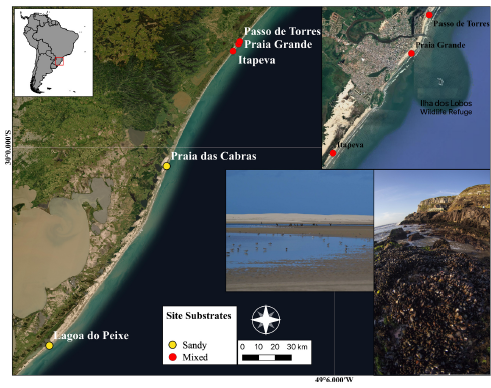
\includegraphics[width=5in,height=\textheight]{fig1.png}

}

\caption{\label{fig-first}Breeding sites of the American oystercatcher
(Haematopus palliatus) along the southern Brazilian coast. Rocky
substrate with Perna perna near to Praia Grande (red arrow); fore dunes
and mudflats at Lagoa do Peixe (yellow arrow). Photo: Mar Pedro de
Abreu. (For interpretation of the references to colour in this figure
legend, the reader is referred to the web version of this article.)}

\end{figure}

\hypertarget{sec-verify}{%
\section{Results}\label{sec-verify}}

Not sure what will happen here

\hypertarget{sec-conc}{%
\section{Discussion}\label{sec-conc}}

Here we discuss results

\hypertarget{disclosure-statement}{%
\section{Disclosure statement}\label{disclosure-statement}}

No conflicts of interest exist).

\hypertarget{bibtex}{%
\section{BibTeX}\label{bibtex}}

We encourage you to use BibTeX. If you have, please feel free to use the
package natbib with any bibliography style you're comfortable with. The
.bst file agsm has been included here for your convenience.


  \bibliography{bibliography.bib}


\end{document}
